\documentclass[10pt, a4paper]{report}
\usepackage{trymtex}
\usepackage[acronym,symbols,nogroupskip]{glossaries-extra}
\usepackage[backend=biber]{biblatex}

\makeglossaries
\addbibresource{preamble/bib/references.bib}
\setglossarystyle{listhypergroup}

\includeonly{
    preamble/frontmatter/titlepage,
    preamble/bib/glossary,
    chapters/1_Introduction,
    % chapters/2_UnconstrainedOptimization,
    % chapters/3_ConvexOptimization,
    % preamble/appendix/AlgorithmMap,
    % preamble/appendix/Formulas,
    % preamble/appendix/Functions,
    preamble/appendix/LectureNotes,
}
\begin{document}
\include{preamble/bib/glossary}
\begin{titlepage}
    \newcommand{\HRule}{\rule{\linewidth}{0.5mm}}
    
    \center
    
    \vspace*{5cm}
    
    % Course code & title
    {\color{ntnu-blue}\sffamily\huge\bfseries TMA4180 \par}
    \vspace{0.5cm}
    {\sffamily\Huge\bfseries Optimering I \par}
    
    \vspace{1.5cm}
    
    \HRule
    \vspace{0.5cm}
    
    % Course notes title
    {\Large\sffamily Notater i Optimering I \par}
    
    \vspace{0.5cm}
    \HRule
    
    \vspace{2cm}
    
    % Author info
    \begin{minipage}{0.4\textwidth}
        \begin{flushleft}
            \large
            \textbf{Author:}\\
            Trym Sæther\\
            \vspace{0.3cm}
            \includegraphics[height=1cm]{frontmatter/signature.png}\\
            \vspace{0.3cm}
            \textit{Physics and Mathematics}
        \end{flushleft}
    \end{minipage}
    ~
    \begin{minipage}{0.4\textwidth}
        \begin{flushright}
            \large
            \textbf{Semester:}\\
            Spring 2025\\
            6th semester
        \end{flushright}
    \end{minipage}
    
    \vfill
    
    % University logo/name
    \begin{center}
        {\color{ntnu-blue}\sffamily\Large Norwegian University of Science and Technology}\\
        \vspace{0.3cm}
        {\sffamily\large Department of Mathematical Sciences}
    \end{center}
    
    \vspace{1cm} 
\end{titlepage}

\tableofcontents

\clearpage

\part{Optimeringsproblemer og Optimalitet}
\label{part:introduction}
\chapter{Forhåndskunnskaper}
\label{chap:mathematical_background}

\section{Vektorrom og produkter}

\subsection{Ytre og indre produkter}
\begin{definition}{Ytre produkt}{outer_product}
	Gitt to vektorer \( \symbf{a} \in \R^m \) og \( \symbf{b} \in \R^n \), er det ytre produktet definert som:
	\[
		\symbf{a} \otimes \symbf{b} = \symbf{a} \symbf{b}^\top =
		\begin{bmatrix}
			a_1b_1 & a_1b_2 & \cdots & a_1b_n \\
			a_2b_1 & a_2b_2 & \cdots & a_2b_n \\
			\vdots & \vdots & \ddots & \vdots \\
			a_mb_1 & a_mb_2 & \cdots & a_mb_n
		\end{bmatrix}
	\]
\end{definition}

\begin{definition}{Indre produkt}{inner_product}
	Gitt to vektorer \( \symbf{a}, \symbf{b} \in \R^n \), er det indre produktet definert som:

	\[
		\symbf{a} \cdot \symbf{b} = \symbf{a}^\top \symbf{b} = \sum_{i=1}^{n} a_i b_i
	\]

\end{definition}

\section{Mengder}

\subsection{Baller}
En åpen ball i \(\R^d\) er en mengde av punkter \(\mathbf{x}\) som ligger innenfor en viss avstand \(r\) fra et sentrum \(\mathbf{x_0}\).

Den er definert ved hjelp av den euklidiske normen \(\norm{\cdot}\), som måler avstanden mellom to punkter i rommet.

\begin{definition}{Åpen Ball}{open_ball}
	En åpen ball \(B(\mathbf{x}_0, r)\) i \(\R^d\) med sentrum \(\mathbf{x_0}\) og radius \(r\) er definert som:
	\[
		B(\mathbf{x}_0, r) = \{ \mathbf{x} \in \R^d : \norm{\mathbf{x} - \mathbf{x}_0} < r\}
	\]
	\begin{itemize}
		\item \(B(\mathbf{x}_0, r)\) er åpen hvis den ikke inkluderer grensen.
		\item \(B(\mathbf{x}_0, r)\) er lukket hvis den inkluderer grensen.
	\end{itemize}
\end{definition}

\subsection{Nivåsett}
Intuitivt er nivåsettet til en funksjon \( f \) i et punkt \( y \) mengden av alle punkter \( x \) som har samme eller lavere verdi enn \( y \) under \( f \).
\begin{definition}{Nivåsett}{level_set}
	\(f: \Omega \to \overline{\R}\) er en funksjon. Vi definerer nivåsettet til \(f\) i punktet \(y \in \R\) som:
	\[
		\mathcal{L}_f(y) = \{x \in \Omega | f(x) = y\}.
	\]
\end{definition}

\subsection{Åpen mengde}

\begin{definition}{Åpen mengde}{open_set}
	En mengde \(A \subset \R^n\) er åpen hvis for alle \(x \in A\) finnes det en \(\varepsilon > 0\) slik at \(B(x, \varepsilon) \subset A\).
	\[
		\forall x \in A, \exists \varepsilon > 0 \text{ s.a. } B(x, \varepsilon) \subset A
	\]
\end{definition}

\subsection{Lukket mengde}
\begin{definition}{Lukket mengde}{closed_set}
	En mengde \(A \subset \R^n\) er lukket hvis komplementet \(A^c\) er åpent.
	\[
		A \text{ er lukket} \Leftrightarrow A^c \text{ er åpen}
	\]
\end{definition}

\subsection{Begrenset mengde}

En mengde er begrenset hvis den ikke strekker seg til uendelig langt i noen retning.
Intuitivt kan vi si at en mengde er begrenset hvis den kan plasseres innenfor en kule med endelig radius.

\begin{definition}{Begrenset mengde}{bounded_set}
	En mengde \(A \subset \R^n\) er begrenset hvis det finnes en \(R > 0\) slik at
	\[
		\norm{x} \leq R \quad \forall x \in A
	\]
\end{definition}

\subsection{Kompakt mengde}

En kompakt mengde er en mengde som er både lukket og begrenset. Dette betyr at den er avgrenset og inneholder alle sine grenseverdier.

\begin{definition}{Kompakt mengde}{compact_set}
	En mengde \(A \subset \R^n\) er kompakt hvis den er lukket og begrenset.
	\[
		A \text{ er kompakt} \Leftrightarrow A \text{ er lukket og begrenset}
	\]
\end{definition}

\section{Funksjoner}
\subsection{Nedre semi-kontinuerlige funksjoner}
En nedre semikontinuerlig funksjon (\textit{lower semi-continuous function}) er en funksjon som ikke har plutselige "hopp nedover".

Tenk deg at du nærmer deg et punkt \( \symbf{x_0} \) fra alle mulige retninger:
\begin{itemize}
	\item Verdien av funksjonen i \( \symbf{x_0} \) vil ikke være høyere enn verdiene du ser når du kommer nærmere.
	\item Funksjonen kan ha "hopp oppover".
\end{itemize}


\begin{definition}{Nedre semi-kontinuerlig funksjoner}{lsc}
	\(f: \Omega (\subset \R^d) \to \overline{\R}\) være en funksjon. Vi sier at \(f\) er nedre semi-kontinuerlig (lsc) i punktet \(x_0\) hvis for alle \(\varepsilon > 0\) finnes det en \(\delta > 0\) slik at
	\[
		f(x) > f(x_0) - \varepsilon \quad \text{for alle} \quad x \in B(x_0, \delta).
	\]
	\begin{enumerate}
		\item \(f\) er (lsc) i \(x_0\) hvis det for alle \(\alpha \in \R\) er mengden \(\mathcal{L}_f(\alpha) = \{x | f(x) < \alpha \} \text{ er åpen i } \R^d\)
		\item \(f\) er (lsc) i \(x_0 \in X\) hvis og bare hvis: \(\liminf_{x \to x_0} f(x) \geq f(x_0)\).
	\end{enumerate}
\end{definition}
\begin{example}{Eksempel på en nedre semi-kontinuerlig funksjon}{lsc}
	\includegraphics[width=0.5\textwidth]{figures/example_lsc.png}
\end{example}

\subsection{Koersivitet}
En koersiv funksjon er intuitivt en funksjon som "går mot uendelig" når vi beveger oss mot kanten av definisjonsmengden hvor \( f \) er definert.

\begin{definition}{Koersivitet}{coercive}
	En funksjon \(f: \Omega \to \R\) er koersiv hvis for alle \(y \in \R\) er nivåmengden \(\mathcal{L}_f(y) = \{x \in \Omega | f(x) \leq y\}\) kompakt.

	\[
		\lim_{\norm{x} \to +\infty} f(x) = +\infty
	\]
\end{definition}

\subsection{Konveksitet, kvasi-konveksitet og konvekse mengder}

Konveksitet er et viktig begrep i optimering og matematikk generelt. Det refererer til formen på en funksjon eller en mengde.
\begin{itemize}
	\item En konveks funksjon har en bue som vender oppover.
	\item En konkav funksjon har en bue som vender nedover.
	\item En konveks mengde er en mengde der enhver linje mellom to punkter i mengden også ligger helt innenfor mengden.
\end{itemize}

\begin{definition}{Konveks funksjon}{convex_function}
	En funksjon \(f: \R^n \to \R\) er konveks hvis for alle \(x, y \in \R^n\) og \(\lambda \in [0, 1]\) har vi:

	\begin{align*}
		f(\lambda x + (1 - \lambda)y) & \leq \lambda f(x) + (1 - \lambda)f(y) \\
	\end{align*}
\end{definition}

\begin{definition}{Strengt konveks funksjon}{strictly_convex}
	En funksjon \(f: \R^n \to \R\) er strengt konveks hvis for alle \(x, y \in \R^n\) og \(\lambda \in (0, 1)\) har vi:
	\[
		f(\lambda x + (1 - \lambda)y) < \lambda f(x) + (1 - \lambda)f(y)
	\]
\end{definition}

\begin{remark}{Konveksitet med indre-produkt notasjon}{convex_inner_product}
	En funksjon  \(f: \R^n \to \R\) er konveks hvis og bare hvis:
	\[
		f(y) - f(x) \geq  \langle \nabla f(x), y - x \rangle
	\]
	for alle  \(x, y \in \R^n\).
\end{remark}


\begin{remark}{Kvasi-konveks}{quasi_convex}
	En funksjon \(f: \R^d \to \R\) er kvasi-konveks hvis for alle \(x, y \in \R^n\) og \(\lambda \in (0, 1)\) har vi:

	\[
		f(\lambda x + (1 - \lambda)y) \leq \max\{f(x), f(y)\}
	\]

	En alternativ definisjon er at en funksjon er kvasi-konveks hvis alle nivåsettene er konvekse.

	\[
		\mathcal{L}_f(y) = \{x \in \R^n | f(x) \leq y\} \quad \text{er konveks for alle} \quad y \in \R
	\]

	\[
		\boxed{\underbrace{\forall \alpha \in \R, \mathcal{L}_f(\alpha) \text{ er konveks}}_{f \text{ er kvasi-konveks }}\Longleftrightarrow \forall x, y \in \R^d,\lambda \text{ s.a. } f(\lambda x + (1-\lambda)y) \leq \max \{ f(x), f(y) \}}
	\]
\end{remark}

\begin{definition}{Konveks sett}{convex_set}
	En mengde \(C \subset \R^n\) er (strengt) konveks når:

	\begin{align*}
		\lambda x + (1 - \lambda)y & \in C \quad \forall \; x, y \in C, \lambda \in [0, 1] \tag{Konveks}                   \\
		\lambda x + (1 - \lambda)y & \in C \quad \forall \; x, y \in C, \lambda \in (0, 1), x \neq y \tag{Strengt konveks}
	\end{align*}

\end{definition}

\begin{definition}{Konveks kombinasjon}{convex_combination}
	En konveks kombinasjon av punkter $x_1, x_2, \ldots, x_n$ i $\mathbb{R}^d$ er ethvert punkt på formen:
	\[
		\sum_{i=1}^n \lambda_i x_i \quad \text{der} \quad \lambda_i \geq 0, \sum_{i=1}^n \lambda_i = 1
	\]
\end{definition}

\begin{remark}{Karakterisering av deriverbare konvekse funksjoner}{convex-characterization}
	For en deriverbar funksjon  \(f: \R^n \to \R\) er følgende ekvivalente:
	\begin{itemize}
		\item  \(f\) er konveks
		\item For alle  \(x, y \in \R^n\) gjelder:
		      \[
			      f(y) \geq f(x) + \nabla f(x)^\top (y - x)
		      \]
	\end{itemize}
\end{remark}

\section{Geometriske objekter}
\subsection{Simplex}
Et simplex er en geometrisk figur som kan forstås som den enkleste formen i et gitt antall dimensjoner. For eksempel er et 0-simplex et punkt, et 1-simplex er en linje, et 2-simplex er en trekant, og så videre.

\begin{definition}{Simplex}{simplex}
	Et simplex i \( \mathbb{R}^n \) er et \( n \)-dimensjonalt objekt laget av \( n+1 \) punkter (hjørner) som ikke ligger i samme hyperplan.

	\begin{figure}[H]
		\centering
		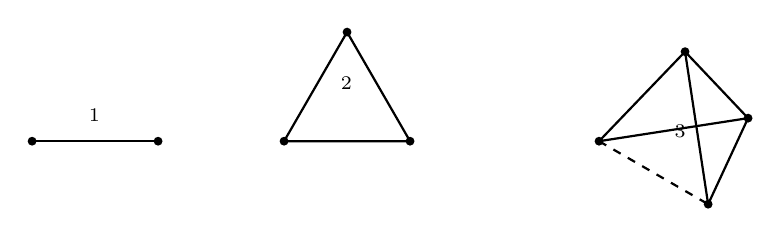
\begin{tikzpicture}[scale=0.8]
			% R1 simplex (line)
			\begin{scope}[shift={(-4,0)}]
				\draw[thick] (0,0) -- (2,0);
				\fill (0,0) circle (2pt);
				\fill (2,0) circle (2pt);
				\node[above] at (1,0) {$\R^1$};
			\end{scope}

			% R2 simplex (triangle)
			\begin{scope}[shift={(0,0)}]
				\draw[thick] (0,0) -- (2,0) -- (1,1.732) -- cycle;
				\fill (0,0) circle (2pt);
				\fill (2,0) circle (2pt);
				\fill (1,1.732) circle (2pt);
				\node[above] at (1,0.5) {$\R^2$};
			\end{scope}

			% R3 simplex (tetrahedron)
			\begin{scope}[shift={(5,0)}, x={(0.866cm,-0.5cm)}, y={(0.866cm,0.5cm)}, z={(0cm,1cm)}]
				% Back triangle
				\draw[thick,dashed] (0,0,0) -- (2,0,0);
				\draw[thick] (2,0,0) -- (1,1.732,0) -- (0,0,0);
				% Vertical edges to top point
				\draw[thick] (0,0,0) -- (1,0.577,1.633);
				\draw[thick] (2,0,0) -- (1,0.577,1.633);
				\draw[thick] (1,1.732,0) -- (1,0.577,1.633);
				% Points
				\fill (0,0,0) circle (2pt);
				\fill (2,0,0) circle (2pt);
				\fill (1,1.732,0) circle (2pt);
				\fill (1,0.577,1.633) circle (2pt);
				\node[above] at (1,0.5,0) {$\R^3$};
			\end{scope}
		\end{tikzpicture}
		\caption{Simplex i ulike dimensjoner.}
	\end{figure}
\end{definition}

\chapter{Hva er optimering?}
\label{chap:what_is_optimization}

Optimering er et felt innen matematikken som handler om å finne den beste løsningen på et gitt problem, enten med eller uten restriksjoner på løsningsrommet.

Målet i et \emph{optimeringsproblem} er å finne en variabel \(x^\star \in \Omega\) som minimerer eller maksimerer en gitt funksjon \(f: \Omega \to \R\), 
kalt \emph{mål\-funksjonen} eller \emph{kostnads\-funksjonen}.

\section{Optimeringsproblemer i \texorpdfstring{\(\R^d\)}{Rd}}

Mengden \(\Omega \subseteq \R^d\) betegner de tillatte løsningene og kalles ofte \emph{søkeområdet} eller den \emph{tillatte mengden (eng. feasible set)}.

\begin{definition}{Optimeringsproblemet \((P)\)}{def:optimization_problem}

	La \(f: \Omega \to \R\) være en funksjon vi ønsker å minimere eller maksimere, der \(\Omega \subseteq \R^d\) er mengden av tillatte (mulige) løsninger.
	\[
		\min_{x \in \Omega} f(x) \quad \text{eller} \quad \max_{x \in \Omega} f(x) \tag{P}
	\]

\end{definition}

Vi fokuserer hovedsakelig på minimeringsproblemer, siden maksimeringsproblemer enkelt kan omformuleres ved å erstatte \(f(x)\) med \(-f(x)\). 
De fleste algoritmene vi diskuterer, er designet for å løse minimeringsproblemer.

\section{Ubundet og Bundet optimering}
Ulike problemtyper oppstår ut fra hvordan denne mengden \(\Omega\) er definert, og hvilke egenskaper funksjonen \(f\) har. Nedenfor gir vi en oversikt over de mest sentrale klassene av optimeringsproblemer:

\begin{itemize}
	\item \textbf{Ubundet optimering}: Dette er den enkleste typen, uten eksplisitte restriksjoner på variabelen \(x\). Her er \(\Omega = \R^d\), og vi søker å minimere \(f(x)\) over hele rommet.
	\item \textbf{Betinget optimering}: Her pålegges løsningen restriksjoner, og den tillatte mengden \(\Omega \subset \R^d\) er definert ved:
	\[
		\Omega = \{ x \in \R^d \mid g_i(x) \leq 0, \, i \in \mathcal{I}, \quad h_j(x) = 0, \, j \in \mathcal{E} \}.
	\]
	\begin{itemize}
		\item \textbf{Lineær programmering (LP)}: Når \(f\) og restriksjonene er lineære.
		\item \textbf{Ikke-lineær programmering (NLP)}: Når én eller flere av \(f\), \(g_i\), eller \(h_j\) er ikke-lineære.
		\item \textbf{Kvadratisk programmering (QP)}: Når \(f\) er kvadratisk og restriksjonene er lineære.
	\end{itemize}
	\item \textbf{Konveks optimering}: En spesialklasse der \(f\) og \(\Omega\) er konvekse. 
	Dette forteller oss at enhver lokal løsning er global, løsningen er entydig hvis \(f\) er strengt konveks, og effektive algoritmer finnes.
\end{itemize}

\section{Globale og lokale løsninger}
\label{sec:global_and_local_solutions}
I optimeringsproblemer er det viktig å skille mellom globale og lokale løsninger. En global løsning er den beste løsningen i hele søkeområdet, mens en lokal løsning er den beste løsningen i et begrenset område rundt et punkt.


\subsection{Globale løsninger}
En global løsning er den beste løsningen i hele søkeområdet \(\Omega\). Dette betyr at det ikke finnes noen annen løsning i hele \(\Omega\) som gir en bedre verdi for funksjonen \(f\).

\begin{definition}{Globale løsninger}{global_solution}

	\medskip
	For en funksjon \(f: \Omega \to \R\) sier vi at \(\symbf{x}^\star \in \Omega\) er en global løsning av minimeringsproblemet~\eqref{eq:global_minimization_problem} hvis:

	\begin{align*}
		f(\symbf{x}^\star) & \leq f(\symbf{x}) \quad \forall \symbf{x} \in \Omega \tag{Global}                                      \\
		f(\symbf{x}^\star) & < f(\symbf{x}) \quad \forall \symbf{x} \in \Omega, \symbf{x} \neq \symbf{x}^\star \tag{Strengt Global}
	\end{align*}
\end{definition}

\subsubsection{Eksistens av globale løsninger}

En funksjon \(f: \Omega \subset \R^d \to \overline{\R}\) har en global løsning (minimum) i \(\Omega\) hvis den er:

\begin{itemize}
	\item \textbf{Nedre semi-kontinuerlig}: For alle \(x \in \Omega\) og alle sekvenser \((x_n)\) som konvergerer mot \(x\):
	      \[
		      f(x) \leq \liminf_{n \to \infty} f(x_n).
	      \]
	\item \textbf{Koersiv}: Det finnes en konstant \(M > 0\) slik at
	      \[
		      f(x) \geq M \quad \forall x \in \Omega.
	      \]
	      Dette sikrer at \(f\) ikke går mot \(-\infty\) når \(x\) går mot uendelig.
\end{itemize}

\begin{theorem}{Eksistens av globale løsninger}{existence_of_global_solution}
	La \(f: \Omega \subset \R^d \to \overline{\R}\) være nedre semi-kontinuerlig og koersiv på \(\Omega\). Da har \(f\) en global løsning (minimum) i \(\Omega\).
\end{theorem}

\subsection{Lokale løsninger}
En lokal løsning er den beste løsningen i et begrenset område rundt et punkt \(\symbf{x}^\star\).
For å avgjøre om \(\symbf{x}^\star\) er en lokal løsning, må vi undersøke om det finnes bedre løsninger i nærheten. 
De fleste metoder for dette baseres på Taylor-utvikling \ref{thm:taylor_theorem}.


\begin{definition}{Lokal løsning}{}
	La \(f: \Omega \to \R\) være en funksjon.

	Vi sier at \(x^\star \in \Omega\) er en lokal løsning av optimeringsproblemet hvis, for en viss \(\varepsilon > 0\):

	\begin{align*}
		f(\symbf{x}^\star) & \leq f(\symbf{x}) \quad \forall \; \symbf{x} \in B(\symbf{x}^\star, \varepsilon) \cap \Omega,                                                  \\
		f(\symbf{x}^\star) & < f(\symbf{x}) \quad \forall \; \symbf{x} \in B(\symbf{x}^\star, \varepsilon) \cap \Omega, \symbf{x} \neq \symbf{x}^\star. \tag{Strengt lokal}
	\end{align*}

	hvor \(B(\symbf{x}^\star, \varepsilon)\) er en åpen kule med sentrum \(\symbf{x}^\star\) og radius \(\varepsilon\)~\ref{def:open_ball}.
\end{definition}

\subsubsection{Taylors teorem}
Taylor-utvikling er en metode for å tilnærme en funksjon ved hjelp av dens deriverte.
Den gir oss en måte å uttrykke funksjonen som en sum av dens verdier og deriverte i et punkt, noe som kan være nyttig for å analysere oppførselen til funksjonen i nærheten av det punktet.

Ved hjelp av Taylor-utvikling kan vi avgjøre om \(\symbf{x}^\star\) er en lokal løsning ved å sjekke om gradienten \(\nabla f(\symbf{x}^\star) = 0\) og Hesse-matrisen \(\nabla^2 f(\symbf{x}^\star)\)

\begin{theorem}{Taylors teorem}{taylors_theorem}
	Anta at \(f: \R^n \to \R\) med \(\mathbf{p}\in\R^n\), og la \(t\in[0,1]\).

	\medskip

	Hvis \(f\in\Ccal^1\) (én gang kontinuerlig deriverbar):
	\[
		f(\mathbf{x} + \mathbf{p}) = f(\mathbf{x}) + \nabla f(\mathbf{x}+t\mathbf{p})^\top \mathbf{p},
	\]

	Hvis \(f \in \Ccal^2\) (to ganger kontinuerlig deriverbar):

	\begin{align*}
		\nabla f(\mathbf{x} + \mathbf{p}) = \nabla f(\mathbf{x}) + \int_0^1 \nabla^2 f(\mathbf{x}+t\mathbf{p})\mathbf{p} dt, \\
		\boxed{f(\mathbf{x} + \mathbf{p}) = f(\mathbf{x}) + \nabla f(\mathbf{x})^\top \mathbf{p} + \frac{1}{2}\mathbf{p}^\top \nabla^2 f(\mathbf{x}+t\mathbf{p})\mathbf{p}}
	\end{align*}
\end{theorem}

\subsubsection{Isolerte lokale løsninger}
En isolert lokal løsning er en lokal løsning der det ikke finnes andre løsninger i nærheten. Dette betyr at det er en viss avstand fra \(\symbf{x}^\star\) til alle andre løsninger.

\begin{lemma}{Isolert lokal løsning}{isolated_local_solution}
	La \(f: \Omega \to \R\) være en funksjon.

	Hvis \(\symbf{x}^\star \in \Omega\) er en isolert lokal løsning, finnes det en \(\varepsilon > 0\) slik at:

	\[
		f(\symbf{x}^\star) \leq f(\symbf{x}) \quad \forall \; \symbf{x} \in B(\symbf{x}^\star, \varepsilon) \cap \Omega, \symbf{x} \neq \symbf{x}^\star.
	\]
\end{lemma}

\chapter{Optimalitetsbetingelser}
\label{chap:optimality_conditions}
\section{Første Ordens Nødvendige Betingelser}

For en lokal løsning \(\mathbf{x}^\star\) må gradienten være null:

\begin{theorem}{First-Order Necessary Conditions}{first_order_necessary_conditions}
	Hvis \(\mathbf{x}^\star\) er et lokalt minimum, og \(f\) er kontinuerlig deriverbar rundt \(\mathbf{x}^\star\), da er:
	\[
		\nabla f(\mathbf{x}^\star) = 0.
	\]
\end{theorem}

\section{Andre Ordens Nødvendige Betingelser}

For en lokal løsning må både gradienten være null og Hesse-matrisen positiv definit:

\begin{theorem}{Second-Order Necessary Conditions}{second_order_necessary_conditions}
	Hvis \(\mathbf{x}^\star\) er et lokalt minimum, og \(f\) er to ganger kontinuerlig deriverbar rundt \(\mathbf{x}^\star\), da er:
	\[
		\nabla f(\mathbf{x}^\star) = 0 \quad \text{og} \quad \nabla^2 f(\mathbf{x}^\star) \succeq 0.
	\]
\end{theorem}

\section{Andre Ordens Tilstrekkelige Betingelser}

\begin{theorem}{Second-Order Sufficient Conditions}{second_order_sufficient_conditions}
	Hvis \(\nabla f(\mathbf{x}^\star) = 0\) og \(\nabla^2 f(\mathbf{x}^\star) \succ 0\) (positiv definit), da er \(\mathbf{x}^\star\) et \emph{strengt lokalt minimum}.

	\medskip

	Det vil si at det finnes en \(\varepsilon > 0\) slik at:
	\[
		f(\mathbf{x}^\star) < f(\mathbf{x})  \quad \forall \; \mathbf{x} \in B(\mathbf{x}^\star, \varepsilon) \cap \Omega, \mathbf{x} \neq \mathbf{x}^\star.
	\]
\end{theorem}

\section{Stasjonære punkter}
Stasjonære punkter er punkter der gradienten til funksjonen er null. Dette betyr at det ikke er noen retning der funksjonen øker eller minker, og det kan være et minimum, maksimum eller et sadelpunkt.

\begin{definition}{Stasjonære punkter}{stationary_points}
	La \(f: \Omega \to \R\) være en funksjon. Et punkt \(\symbf{x}^\star \in \Omega\) er et stasjonært punkt hvis:
	\[
		\nabla f(\symbf{x}^\star) = 0.
	\]
	Dette betyr at gradienten til \(f\) i punktet \(\symbf{x}^\star\) er lik null.
\end{definition}

\subsection{Konvergens til stasjonære punkter}
Når vi bruker iterative metoder for å finne minimum av en funksjon \(f\), ønsker vi å vite om algoritmen vil konvergere til det stasjonære punktet \(\symbf{x}^\star\).

\begin{theorem}{Konvergens til stasjonære punkter}{convergence_to_stationary_points}
	Anta at \(f: \R^d \to \R\) er en kontinuerlig deriverbar funksjon, og at følgende betingelser er oppfylt:
	\begin{enumerate}
		\item \(\Omega\) er en lukket og begrenset mengde.
		\item \(f(\symbf{x})\) er koersiv.
		\item \(f(\symbf{x})\) er nedre semi-kontinuerlig.
		\item \(\nabla f(\symbf{x})\) eksisterer og er Lipschitz-kontinuerlig.
		\item \(\nabla^2 f(\symbf{x})\) eksisterer og er Lipschitz-kontinuerlig.
	\end{enumerate}
	Da konvergerer sekvensen \((\symbf{x}_k)\) generert av en optimaliseringsalgoritme til et stasjonært punkt \(\symbf{x}^\star\) i \(\Omega\).
	\[
		\lim_{k \to \infty} \|\nabla f(\symbf{x}_k)\| = 0.
	\]
	
	hvor \(\symbf{x}_k\) er iteratene generert av en optimaliseringsalgoritme, og \(\symbf{x}^\star\) tilfredsstiller de førsteordens nødvendige betingelsene \(\nabla f(\symbf{x}^\star) = 0\).

\end{theorem}

\section{Optimalitet og konveksitet}
\label{sec:optimality_and_convexity}
For en konveks funksjon \(f\) er det stasjonære punktet \(\mathbf{x}^\star\) også et globalt minimum. Dette er en viktig egenskap ved konvekse funksjoner, og det gjør dem spesielt nyttige i optimering.

\begin{remark}{Konveksitet og stasjonære punkter}{convexity_and_stationary_points}
	\begin{itemize}
		\item Hvis \(f\) er \textbf{konveks} så er alle lokale minimum \(\mathbf{x}^\star\) også globale minimum.
		\item Hvis \(f\) er \textbf{konveks} og \textbf{deriverbar} så er alle stasjonære punkter \(\mathbf{x}^\star\) også globale minimum.
	\end{itemize}
\end{remark}

\begin{example}{Eksistens og optimalitet}{}
		For \( f(x) = x^2 + 2x \), som er kontinuerlig og koersiv, finnes et globalt minimum i \( x^* = -1 \) der \( f(-1) = -1 \).
\end{example}
\begin{example}{Eksistens og optimalitet}{}
			
	For \( f(x) = x^2 \), har vi \( \nabla f(x) = 2x \). I \( x^* = 0 \) er \( \nabla f(0) = 0 \) og \( \nabla^2 f(x) = 2 > 0 \), som oppfyller SOSC.

\end{example}





\chapter{Ubundet Optimalisering}\label{chap:unconstrained_optimization}

Ubundet optimalisering (eller fri optimalisering) refererer til problemer uten eksplisitte restriksjoner på variablene.
Målet er å minimere en \textit{glatt objektfunksjon} \( f : \mathbb{R}^n \to \mathbb{R} \) over hele \(\mathbb{R}^n\):

\[
  \min_{\symbf{x} \in \mathbb{R}^n} f(\symbf{x}),
\]

hvor løsningen \(\symbf{x}^*\) tilfredsstiller

\[
  f(\symbf{x}^*) \;\le\; f(\symbf{x})
  \quad \forall \symbf{x} \in \mathbb{R}^n.
\]

\paragraph{Egenskaper ved ubundet optimalisering}

\begin{itemize}
  \item \textbf{Ingen restriksjoner}: Den tillatte mengden (feasible set) er hele \(\mathbb{R}^n\), uten likhets- eller ulikhetsbetingelser.
  \item \textbf{Enklere oppsett}: Det er ikke behov for å håndtere restriksjoner i selve problemet.
  \item \textbf{Fokuserer kun på målfunksjonen}: Algoritmer søker etter punkter \(\symbf{x}\) som reduserer \(f(\symbf{x})\) direkte, uten å ta hensyn til andre forhold.
\end{itemize}

\section{Stasjonære punkter}\label{sec:stationary_points}

\begin{definition}{Stasjonære punkter}{stationary_points}
  Et punkt \(\symbf{x}^*\) er et stasjonært punkt for \(f\) dersom gradienten \(\nabla f(\symbf{x}^*) = 0\).
\end{definition}

\subsection*{Konvergens til stasjonære punkter}
For å sikre konvergens til en stasjonær løsning \(\symbf{x}^*\), må følgende betingelser typisk oppfylles:
\begin{enumerate}
  \item \(f(\symbf{x})\) er kontinuerlig deriverbar (\(C^1\)).
  \item Gradienten \(\nabla f(\symbf{x})\) eksisterer og er Lipschitz-kontinuerlig.
  \item \hyperref[def:level_set]{Nivåsettene} \(\mathcal{L}_f(\alpha)\) er begrenset og lukkede \hyperref[def:compact_set]{(kompakte)}.
\end{enumerate}

Under disse antagelsene sikres konvergens til en stasjonær løsning \(\symbf{x}^*\) der
\(\nabla f(\symbf{x}^*) = 0\).
Dette innebærer at
\[
  \lim_{k \to \infty} \|\nabla f(\symbf{x}_k)\| = 0,
\]
hvor \(\symbf{x}_k\) er iteratene generert av en optimaliseringsalgoritme, og \(\symbf{x}^*\) tilfredsstiller de førsteordens nødvendige betingelsene \(\nabla f(\symbf{x}^*) = 0\).

\section{Trust Region Metoder}

Trust region-metoder er en annen tilnærming til optimalisering. Istedenfor å velge en retning og deretter en steplengde, definerer vi en region hvor vi "stoler på" en approksimasjon av funksjonen.

\begin{definition}{Trust Region}{trust_region}
  Trust region-metoder løser et begrenset optimaliseringsproblem:
  \[
    \min_{p \in \mathbb{R}^n} m_k(p) \quad \text{slik at} \quad \|p\| \leq \Delta_k
  \]
  hvor $m_k$ er en modell (typisk kvadratisk) av $f$ nær $x_k$ og $\Delta_k > 0$ er trust region-radius.
\end{definition}

\subsection{Trust Region Algoritme}

\begin{enumerate}
  \item Velg initial $x_0$ og $\Delta_0 > 0$, sett $k = 0$
  \item Lag en modell $m_k(p)$ nær $x_k$, typisk:
        \[
          m_k(p) = f(x_k) + \nabla f(x_k)^T p + \frac{1}{2}p^T B_k p
        \]
  \item Løs (approksimativt) trust region-delproblemet:
        \[
          p_k = \arg\min_{p \in \mathbb{R}^n} m_k(p) \quad \text{slik at} \quad \|p\| \leq \Delta_k
        \]
  \item Beregn ratioen av faktisk til predikert reduksjon:
        \[
          \rho_k = \frac{f(x_k) - f(x_k + p_k)}{m_k(0) - m_k(p_k)}
        \]
  \item Oppdater $x_k$ og $\Delta_k$ basert på $\rho_k$:
        \begin{itemize}
          \item Hvis $\rho_k$ er stor: aksepter steget og øk $\Delta_k$
          \item Hvis $\rho_k$ er moderat: aksepter steget men behold $\Delta_k$
          \item Hvis $\rho_k$ er liten: avvis steget og reduser $\Delta_k$
        \end{itemize}
\end{enumerate}

\begin{figure}[H]
  \centering
  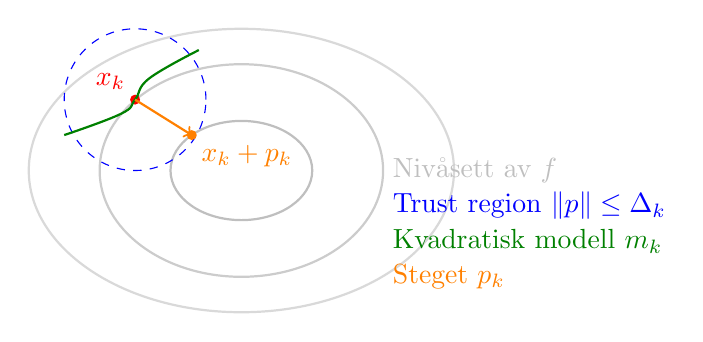
\begin{tikzpicture}[scale=0.9]
    % Contours of the function
    \draw[gray!30, thick] (0,0) ellipse (3 and 2);
    \draw[gray!40, thick] (0,0) ellipse (2 and 1.5);
    \draw[gray!50, thick] (0,0) ellipse (1 and 0.7);

    % Current point
    \fill[red] (-1.5,1) circle (2pt) node[above left]{$x_k$};

    % Trust region
    \draw[blue, dashed] (-1.5,1) circle (1);

    % Model approximation
    \draw[green!50!black, thick] plot[smooth, tension=0.7] coordinates {(-2.5,0.5) (-1.7,0.8) (-1.5,1) (-1.3,1.3) (-0.6,1.7)};

    % Optimal step within trust region
    \draw[->, thick, orange] (-1.5,1) -- (-0.7,0.5);
    \fill[orange] (-0.7,0.5) circle (2pt) node[below right]{$x_k + p_k$};

    % Legend
    \node[gray!50, right] at (2,0) {Nivåsett av $f$};
    \node[blue, right] at (2,-0.5) {Trust region $\|p\| \leq \Delta_k$};
    \node[green!50!black, right] at (2,-1) {Kvadratisk modell $m_k$};
    \node[orange, right] at (2,-1.5) {Steget $p_k$};
  \end{tikzpicture}
  \caption{Trust region-metoden.
    Det blå sirkelen viser det tillatte området (Trust region) rundt $x_k$,
    og det oransje steget er løsningen av delproblemet.}
\end{figure}

\subsection{Trust Region vs. Linjesøk}
\begin{itemize}
  \item \textbf{Trust Region}: Først bestemmes hvor langt vi kan gå (radius $\Delta_k$), deretter bestemmes retningen og steplengden samtidig.
  \item \textbf{Linjesøk}: Først bestemmes retningen $p_k$, deretter bestemmes hvor langt vi skal gå i den retningen (steplengde $\alpha_k$).
\end{itemize}

Trust region-metoder er spesielt robuste når Hessian-matrisen ikke er positiv definit, da de naturlig håndterer negative krumninger ved å begrense steglengden.

\section{Linjesøk}\label{sec:line_search}

Linjesøk er en metode for å finne minimum av en funksjon \(f\) ved å iterere over retninger og steplengder.

Ideen er å velge en retning \(p_k\) og deretter finne en passende steplengde \(\alpha_k\) langs denne retningen.

\begin{definition}{Linjesøk}{line_search}
  Gitt en nåværende iterasjon \(x_k\) og en søkeretning \(p_k\), finner linjesøk en steglengde \(\alpha_k > 0\) slik at
  \[
    x_{k+1} = x_k + \alpha_k p_k
  \]
  gir tilstrekkelig reduksjon i målfunksjonen \(f\).
\end{definition}

For å oppnå dette, må vi oppfylle visse betingelser for \(\alpha_k\).
De varierer i hvor strenge krav de stiller til reduksjonen i funksjonsverdien, gradientens/Hesse-matrisens oppførsel og forholdet mellom disse.
De mest kjente er Wolfe-betingelsene, Armijo-betingelsen, Goldstein-betingelsen, kurvbetingelsen og Strong Wolfe-betingelsene.

\subsection{Wolfe-betingelser}

For å sikre tilstrekkelig forbedring, brukes ofte Wolfe betingelsene:

\begin{align}
  f(x_k + \alpha_k p_k)              & \leq f(x_k) + c_1 \alpha_k \nabla f(x_k)^T p_k \tag{Armijo betingelse} \\
  \nabla f(x_k + \alpha_k p_k)^T p_k & \geq c_2 \nabla f(x_k)^T p_k \tag{Krumningsbetingelse}
\end{align}

der \(0 < c_1 < c_2 < 1\) er konstanter, typisk \(c_1 \approx 10^{-4}\) og \(c_2 \approx 0.9\).

\begin{definition}{Wolfe-betingelsene}{wolfe_conditions}
  \begin{enumerate}
    \item \textbf{Armijo-betingelsen}:
          \[
            f(\symbf{x} + \alpha \symbf{d})
            \;\le\;
            f(\symbf{x})
            \;+\;
            \beta\,\alpha\,\nabla f(\symbf{x})^T \symbf{d}.
          \]
    \item \textbf{Krav til avtagende rate}:
          \[
            \nabla f(\symbf{x} + \alpha \symbf{d})^T \symbf{d}
            \;\ge\;
            \rho \,\nabla f(\symbf{x})^T \symbf{d}.
          \]
  \end{enumerate}
\end{definition}

\subsection{Armijo-betingelsen}
\begin{definition}{Armijo-betingelsen}{armijo_condition}
  Armijo-betingelsen sikrer at steget gir en tilstrekkelig reduksjon i funksjonsverdien. Den krever at
  \[
    f(\symbf{x} + \alpha \symbf{d})
    \;\le\;
    f(\symbf{x})
    \;+\;
    \beta\,\alpha\,\nabla f(\symbf{x})^T \symbf{d},
  \]
  hvor \(\beta\) er en liten positiv konstant. Dette tilsier at \(f\) reduseres i tråd med en lineær modell.
\end{definition}

\begin{figure}[h]
  \centering
  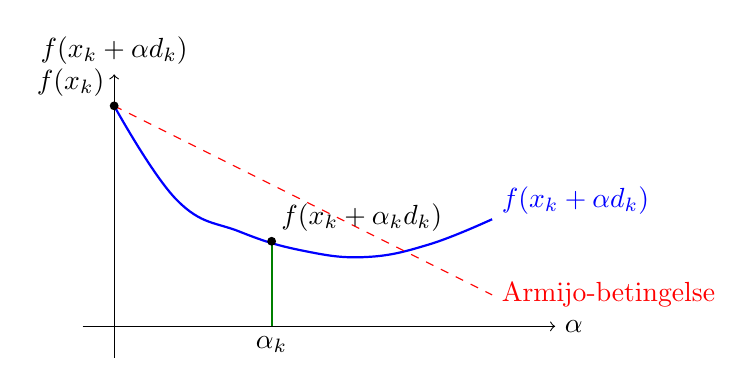
\begin{tikzpicture}[scale=0.8]
    % Axis
    \draw[->] (-0.5,0) -- (7,0) node[right]{$\alpha$};
    \draw[->] (0,-0.5) -- (0,4) node[above]{$f(\symbf{x}_k + \alpha \symbf{d}_k)$};

    % Function curve
    \draw[thick, blue] plot[smooth, tension=0.7] coordinates {(0,3.5) (1,2) (2,1.5) (3,1.2) (4,1.1) (5,1.3) (6,1.7)};

    % Armijo condition line
    \draw[red, dashed] plot coordinates {(0,3.5) (6,0.5)};

    % Initial point
    \fill (0,3.5) circle (2pt) node[above left]{$f(\symbf{x}_k)$};

    % Step point
    \draw[green!50!black, thick] (2.5,0) -- (2.5,1.35);
    \fill (2.5,1.35) circle (2pt) node[above right]{$f(\symbf{x}_k + \alpha_k \symbf{d}_k)$};

    % Step length label
    \node[below] at (2.5,0) {$\alpha_k$};

    % Legend
    \node[blue, right] at (6,2) {$f(\symbf{x}_k + \alpha \symbf{d}_k)$};
    \node[red, right] at (6,0.5) {Armijo-betingelse};
  \end{tikzpicture}
  \caption{Illustrasjon av linjesøk. Den blå kurven viser funksjonen langs søkeretningen, mens den røde stiplede linjen viser Armijo-betingelsen. Steglengden $\alpha_k$ gir tilstrekkelig reduksjon.}
\end{figure}

\subsection{Goldstein-betingelsen}
\begin{definition}{Goldstein-betingelsen}{goldstein_condition}
  Goldstein-betingelsen krever at den nye funksjonsverdien etter steget ligger innenfor et avgrenset intervall:
  \[
    f(\symbf{x}) + (1-\beta)\,\alpha\,\nabla f(\symbf{x})^T \symbf{d}
    \;\le\;
    f(\symbf{x} + \alpha \symbf{d})
    \;\le\;
    f(\symbf{x}) + \beta\,\alpha\,\nabla f(\symbf{x})^T \symbf{d}.
  \]
  Dette forhindrer at vi tar et for lite eller for stort steg.
\end{definition}

\subsection{Kurvbetingelsen}
\begin{definition}{Curvature-betingelsen}{curvature_condition}
  Kurvbetingelsen ser på gradientens endring etter steget og krever
  \[
    \bigl|\nabla f(\symbf{x} + \alpha \symbf{d})^T \symbf{d}\bigr|
    \;\le\;
    -\sigma \,\nabla f(\symbf{x})^T \symbf{d},
  \]
  for en konstant \(\sigma \in (0,1)\). Dette sikrer at gradienten ikke endrer retning for brått, og at man unngår “overkorrigering”.
\end{definition}

\subsection{Strong Wolfe-betingelsene}
\begin{definition}{Strong Wolfe-betingelsene}{strong_wolfe_conditions}
  Strong Wolfe-betingelsene kombinerer Armijo-betingelsen med en kurvbetingelse:
  \begin{enumerate}
    \item Armijo-betingelsen:
          \[
            f(\symbf{x} + \alpha \symbf{d})
            \;\le\;
            f(\symbf{x})
            \;+\;
            \beta\,\alpha\,\nabla f(\symbf{x})^T \symbf{d}.
          \]
    \item Kurvbetingelsen:
          \[
            \bigl|\nabla f(\symbf{x} + \alpha \symbf{d})^T \symbf{d}\bigr|
            \;\le\;
            -\sigma \,\nabla f(\symbf{x})^T \symbf{d}.
          \]
  \end{enumerate}
\end{definition}

\subsection{Goldstein-Wolfe-betingelsene}
\begin{definition}{Goldstein-Wolfe-betingelsene}{goldstein_wolfe_conditions}
  Goldstein-Wolfe-betingelsene krever at Armijo- og Goldstein-betingelsene begge er oppfylt:
  \begin{enumerate}
    \item Armijo-betingelsen:
          \[
            f(\symbf{x} + \alpha \symbf{d})
            \;\le\;
            f(\symbf{x})
            \;+\;
            \beta\,\alpha\,\nabla f(\symbf{x})^T \symbf{d}.
          \]
    \item Goldstein-betingelsen:
          \[
            f(\symbf{x}) + (1-\beta)\,\alpha\,\nabla f(\symbf{x})^T \symbf{d}
            \;\le\;
            f(\symbf{x} + \alpha \symbf{d})
            \;\le\;
            f(\symbf{x}) + \beta\,\alpha\,\nabla f(\symbf{x})^T \symbf{d}.
          \]
  \end{enumerate}
\end{definition}

\subsection{Eksakt vs Ikke-Eksakt Linjesøk}

\begin{itemize}
  \item \textbf{Eksakt linjesøk}: Finn $\alpha_k$ som minimerer $f(x_k + \alpha p_k)$. Dette er ofte beregningsmessig dyrt.
  \item \textbf{Ikke-eksakt linjesøk}: Finn $\alpha_k$ som gir tilstrekkelig reduksjon, f.eks. ved å oppfylle Wolfe betingelsene.
\end{itemize}

Linjesøk omfatter metoder for å finne en egnet skrittlengde \(\alpha\) eller \(\alpha_k\) i en gitt retning \(\symbf{d}\) som reduserer objektfunksjonen \(f(\symbf{x})\).

\subsection{Backtracking Line Search (BLS)}
Backtracking Line Search er en metode for å finne en passende skrittlengde \(\alpha\) som sikrer en ønsket reduksjon i \(f(\symbf{x})\) langs en retning \(\symbf{d}\).

\subsubsection{Algoritme}
\begin{algorithm}[H]
  \SetAlgoLined
  \KwIn{Startpunkt \( \symbf{x} \), retning \( \symbf{d} \), initial skrittlengde \( \alpha \), \textit{backtracking}-parameter \( \beta \in (0,1) \), \textit{skalering} \( \rho \in (0,1) \)}
  \KwOut{Skrittlengde \( \alpha \)}
  \While{\( f(\symbf{x} + \alpha \symbf{d}) > f(\symbf{x}) + \beta \,\alpha \,\nabla f(\symbf{x})^T \symbf{d} \)}{
    \(\alpha \leftarrow \rho \,\alpha\)
  }
  \caption{Backtracking Line Search (BLS)}
  \label{alg:backtracking_line_search}
\end{algorithm}

\subsection{Konvergens av Linjesøk}
\begin{theorem}{Konvergens av linjesøk}{line_search_convergence}
  Anta at \(f\) er kontinuerlig deriverbar og at det finnes en \(\alpha^* > 0\) slik at
  \[
    f(\symbf{x} + \alpha^* \symbf{d}) < f(\symbf{x}) + \beta\,\alpha^*\,\nabla f(\symbf{x})^T \symbf{d}.
  \]
  Da vil Backtracking Line Search konvergere til en skrittlengde \(\alpha_k\) som tilfredsstiller Armijo-betingelsen.
\end{theorem}

\section{Newtons Metode}\label{sec:newtons_method}

Newtons metode er en iterativ tilnærming for å finne lokale ekstremalpunkter i en funksjon. Den bruker andreordens informasjon (Hesse-matrisen) for å avlede en søkeretning som ofte gir raskere konvergens enn gradientbaserte metoder alene.

\subsection{Algoritme}
Gitt en startverdi \( \symbf{x}_0 \), genererer Newtons metode en sekvens av iterasjoner:
\[
  \symbf{x}_{k+1}
  \;=\;
  \symbf{x}_k
  \;-\;
  [\nabla^2 f(\symbf{x}_k)]^{-1} \,\nabla f(\symbf{x}_k),
\]
der:
\begin{itemize}
  \item \(\symbf{x}_{k+1}\) er neste iterasjon.
  \item \(\nabla f(\symbf{x}_k)\) er gradienten av \(f\) evaluert i \(\symbf{x}_k\).
  \item \(\nabla^2 f(\symbf{x}_k)\) er Hesse-matrisen av \(f\) i \(\symbf{x}_k\).
\end{itemize}

\paragraph{Søkeretning}
Søkeretningen finnes ved:
\[
  \symbf{d}_k
  \;=\;
  -[\nabla^2 f(\symbf{x}_k)]^{-1}\,\nabla f(\symbf{x}_k).
\]
\paragraph{Oppdatering}
\[
  \symbf{x}_{k+1}
  \;=\;
  \symbf{x}_k + \alpha_k \,\symbf{d}_k,
\]
\subparagraph{Skrittlengde}
Skrittlengden \(\alpha_k\) kan finnes ved linjesøk (f.eks.\ Backtracking Line Search).

\begin{algorithm}[H]
  \SetAlgoLined
  \KwIn{Startpunkt \( \symbf{x}_0 \), toleranse \( \epsilon \), maks antall iterasjoner \( K \)}
  \KwOut{Omtrentelig løsning \( \symbf{x}^* \)}
  \For{\( k = 0, 1, 2, \ldots, K\)}{
  Beregn søkeretning:
  \(\symbf{d}_k
  = -[\nabla^2 f(\symbf{x}_k)]^{-1}\,\nabla f(\symbf{x}_k)\)\;
  Finn skrittlengde \(\alpha_k\) (f.eks.\ ved Backtracking Line Search)\;
  Oppdater \(
  \symbf{x}_{k+1}
  = \symbf{x}_k + \alpha_k \symbf{d}_k
  \)\;
  \If{\(\|\nabla f(\symbf{x}_{k+1})\| < \epsilon\)}{
    \Return \(\symbf{x}_{k+1}\)\;
  }
  }
  \caption{Newtons metode}
\end{algorithm}

\subsection{Konvergens av Newtons Metode}
Newtons metode kan konvergere lokalt kvadratisk under visse forutsetninger. La \( f : \mathbb{R}^n \to \mathbb{R} \) være to ganger kontinuerlig deriverbar. Anta at:

\begin{enumerate}
  \item Det finnes et \(\symbf{x}^*\) slik at \(\nabla f(\symbf{x}^*) = 0\).
  \item Hesse-matrisen \(\nabla^2 f(\symbf{x}^*)\) er regulær (invertibel).
  \item \(\nabla^2 f\) er Lipschitz-kontinuerlig i et nabolag rundt \(\symbf{x}^*\); dvs.\ det finnes \( L > 0 \) slik at
        \[
          \| \nabla^2 f(\symbf{x}) - \nabla^2 f(\symbf{y}) \|
          \;\le\;
          L\,\|\symbf{x} - \symbf{y}\|,
        \]
        for alle \(\symbf{x}, \symbf{y}\) i dette nabolaget.
\end{enumerate}

Da kan man vise at for en startverdi \(\symbf{x}_0\) nær \(\symbf{x}^*\), vil Newtons metode konvergere kvadratisk mot \(\symbf{x}^*\).

\begin{proof}{}{}
  La \(\symbf{e}_k = \symbf{x}_k - \symbf{x}^*\) være feilen ved iterasjon \(k\).
  Ved Taylor-utvidelse av gradienten får vi:
  \[
    \nabla f(\symbf{x}_k)
    = \nabla^2 f(\symbf{x}^*)\,(\symbf{x}_k - \symbf{x}^*) + r(\symbf{x}_k),
  \]
  hvor \(\|r(\symbf{x}_k)\|\) er \(\mathcal{O}(\|\symbf{e}_k\|^2)\). Newtons oppdateringsregel er
  \[
    \symbf{x}_{k+1}
    = \symbf{x}_k
    - [\nabla^2 f(\symbf{x}_k)]^{-1}\,\nabla f(\symbf{x}_k).
  \]
  I et lite nabolag av \(\symbf{x}^*\) kan vi anta at
  \(\nabla^2 f(\symbf{x}_k)\approx \nabla^2 f(\symbf{x}^*)\), slik at
  \[
    \symbf{e}_{k+1}
    \;=\; \symbf{x}_{k+1} - \symbf{x}^*
    \;\approx\;
    -[\nabla^2 f(\symbf{x}^*)]^{-1}\,r(\symbf{x}_k).
  \]
  Dermed blir
  \[
    \|\symbf{e}_{k+1}\|
    \;\lesssim\;
    \|[\nabla^2 f(\symbf{x}^*)]^{-1}\|\,
    \|r(\symbf{x}_k)\|
    \;\le\;
    C \|\symbf{e}_k\|^2,
  \]
  for en konstant \(C>0\). Dette illustrerer \textit{kvadratisk konvergens} når \(\symbf{x}_0\) er nært \(\symbf{x}^*\).
\end{proof}

\subsection{Bevis for Kvadratisk Konvergens}
\label{sec:newton_quadratic_convergence}
Argumentet ovenfor kan formuleres mer detaljert ved å vise at feilen \(\|\symbf{e}_{k+1}\|\) er proporsjonal med \(\|\symbf{e}_k\|^2\). Dette er selve definisjonen av kvadratisk konvergens.

\subsection{Kommentarer}
Beviset forutsetter at startverdien \(\symbf{x}_0\) er tilstrekkelig nær \(\symbf{x}^*\). I praksis benyttes ofte modifikasjoner, som for eksempel \textit{dempet Newton} (med linjesøk), for å sikre global konvergens før man oppnår den raske, lokale konvergensfasen.

\subsection{Egenskaper}
\begin{itemize}
  \item \textbf{Kvadratisk konvergens}: Under gitte forutsetninger dobles antall riktige sifre omtrent for hver iterasjon.
  \item \textbf{Krever andreordens deriverbarhet}: \(\nabla^2 f(\symbf{x})\) må eksistere og være invertibel.
  \item \textbf{Beregning kan være kostbar}: Å beregne og invertere \(\nabla^2 f(\symbf{x})\) er dyrt, spesielt i store dimensjoner.
  \item \textbf{Global vs.\ lokal konvergens}: Metoden garanterer ikke nødvendigvis global konvergens uten videre tiltak.
\end{itemize}

\subsection{Modifikasjoner}
\begin{itemize}
  \item \textbf{Dempet Newtons metode}: Benytter en skrittlengde \(\alpha_k\) (linjesøk) for å unngå for store steg.
  \item \textbf{Kvasi-Newton-metoder}: Reduserer kostnader ved å approksimere Hesse-matrisen (f.eks.\ BFGS, DFP).
\end{itemize}


\section{Konjugerte Gradientmetode (CG)}\label{sec:conjugate_gradient}

Konjugert Gradient (CG) metoden er en effektiv iterativ algoritme for å løse lineære ligningssystemer og optimere kvadratiske funksjoner. Den er spesielt nyttig for store, men sparse systemer.

\subsection{Grunnleggende Konsept}
CG-metoden genererer en sekvens av retninger som er konjugerte med hensyn til en symmetrisk, positiv definit matrise. For en kvadratisk funksjon:
\[
  f(\symbf{x}) = \frac{1}{2}\symbf{x}^T\symbf{A}\symbf{x} - \symbf{b}^T\symbf{x} + c,
\]
hvor \(\symbf{A}\) er symmetrisk, positiv definit, søker CG-metoden å løse \(\nabla f(\symbf{x}) = \symbf{A}\symbf{x} - \symbf{b} = \symbf{0}\).

\subsection{CG-algoritme}

\begin{algorithm}[H]
  \SetAlgoLined
  \KwIn{Startpunkt \(\symbf{x}_0\), toleranse \(\epsilon > 0\)}
  \KwOut{Omtrentelig løsning \(\symbf{x}^*\)}
  \(\symbf{r}_0 \gets \symbf{b} - \symbf{A}\symbf{x}_0\) \tcc*{Residual}
  \(\symbf{p}_0 \gets \symbf{r}_0\) \tcc*{Første søkeretning}
  \For{\(k = 0, 1, 2, \ldots\)}{
    \If{\(\|\symbf{r}_k\| < \epsilon\)}{
      \Return \(\symbf{x}_k\) \tcc*{Konvergens oppnådd}
    }
    \(\alpha_k \gets \frac{\symbf{r}_k^T\symbf{r}_k}{\symbf{p}_k^T\symbf{A}\symbf{p}_k}\) \tcc*{Optimal skrittlengde}
    \(\symbf{x}_{k+1} \gets \symbf{x}_k + \alpha_k\symbf{p}_k\) \tcc*{Oppdater løsning}
    \(\symbf{r}_{k+1} \gets \symbf{r}_k - \alpha_k\symbf{A}\symbf{p}_k\) \tcc*{Oppdater residual}
    \(\beta_{k+1} \gets \frac{\symbf{r}_{k+1}^T\symbf{r}_{k+1}}{\symbf{r}_k^T\symbf{r}_k}\) \tcc*{Konjugasjonsparameter}
    \(\symbf{p}_{k+1} \gets \symbf{r}_{k+1} + \beta_{k+1}\symbf{p}_k\) \tcc*{Ny søkeretning}
  }
  \caption{Konjugert Gradient Metode (CG)}
\end{algorithm}

\subsection{Ikke-lineær Konjugert Gradient Metode (Non-Linear CG)}

For generelle ikke-lineære funksjoner tilpasses algoritmen:

\begin{algorithm}[H]
  \SetAlgoLined
  \KwIn{Startpunkt \(\symbf{x}_0\), toleranse \(\epsilon > 0\)}
  \KwOut{Omtrentelig løsning \(\symbf{x}^*\)}
  \(\symbf{g}_0 \gets \nabla f(\symbf{x}_0)\) \tcc*{Gradient}
  \(\symbf{p}_0 \gets -\symbf{g}_0\) \tcc*{Første søkeretning}
  \For{\(k = 0, 1, 2, \ldots\)}{
    \If{\(\|\symbf{g}_k\| < \epsilon\)}{
      \Return \(\symbf{x}_k\) \tcc*{Konvergens oppnådd}
    }
    Finn \(\alpha_k\) ved linjesøk som minimerer \(f(\symbf{x}_k + \alpha\symbf{p}_k)\) \;
    \(\symbf{x}_{k+1} \gets \symbf{x}_k + \alpha_k\symbf{p}_k\) \tcc*{Oppdater løsning}
    \(\symbf{g}_{k+1} \gets \nabla f(\symbf{x}_{k+1})\) \tcc*{Ny gradient}
    Beregn \(\beta_{k+1}\) \tcc*{f.eks. FR eller PR}\;
    \(\symbf{p}_{k+1} \gets -\symbf{g}_{k+1} + \beta_{k+1}\symbf{p}_k\) \tcc*{Ny søkeretning}
  }
  \caption{Ikke-lineær Konjugert Gradient Metode (Non-Linear CG)}
\end{algorithm}

\subsection{Valg av beta-parameter}

Flere formler eksisterer for \(\beta\) i ikke-lineære CG-metoder:
\begin{itemize}
  \item \textbf{Fletcher-Reeves}: \(\beta_{k+1}^{FR} = \frac{\symbf{g}_{k+1}^T\symbf{g}_{k+1}}{\symbf{g}_k^T\symbf{g}_k}\)
  \item \textbf{Polak-Ribière}: \(\beta_{k+1}^{PR} = \frac{\symbf{g}_{k+1}^T(\symbf{g}_{k+1}-\symbf{g}_k)}{\symbf{g}_k^T\symbf{g}_k}\)
  \item \textbf{Hestenes-Stiefel}: \(\beta_{k+1}^{HS} = \frac{\symbf{g}_{k+1}^T(\symbf{g}_{k+1}-\symbf{g}_k)}{\symbf{p}_k^T(\symbf{g}_{k+1}-\symbf{g}_k)}\)
\end{itemize}

\subsection{Egenskaper}
\begin{itemize}
  \item \textbf{Hurtig konvergens}: For kvadratiske funksjoner konvergerer metoden på maksimalt \(n\) iterasjoner (i eksakt aritmetikk), hvor \(n\) er problemdimensjon.
  \item \textbf{Minneeffektivitet}: Lagrer kun et begrenset antall vektorer, noe som gjør den egnet for store problemer.
  \item \textbf{Numerisk stabilitet}: God oppførsel under avrundingsfeil, spesielt med periodisk omstart.
  \item \textbf{Forbehandling}: Kan akselereres videre ved å bruke en prekondisjonerer som transformerer problemet.
\end{itemize}

\subsection{Prekondisjonering}
Konvergenshastigheten kan forbedres ved å bruke en prekondisjonerer \(\symbf{M}\) som approksimerer \(\symbf{A}\) på en inverterbar måte. Den prekondisjonerte algoritmen løser det transformerte systemet:
\[
  \symbf{M}^{-1}\symbf{A}\symbf{x} = \symbf{M}^{-1}\symbf{b}.
\]
Dette reduserer kondisjonstallet og akselererer konvergensen.

\section{Quasi-Newton Metoder}\label{sec:quasi_newton}

Quasi-Newton metoder er en klasse av optimeringsalgoritmer som tilnærmer seg Newtons metode, men unngår det kostbare arbeidet med å beregne Hesse-matrisen direkte. Istedenfor bygger de opp en approksimering av Hesse-matrisen (eller dens invers) ved hjelp av gradient-informasjon fra tidligere iterasjoner.

\subsection{Motivasjon}
Newtons metode krever beregning og invertering av Hesse-matrisen \(\nabla^2 f(\symbf{x})\) i hver iterasjon, noe som er beregningsintensivt for høydimensjonale problemer. Quasi-Newton metoder reduserer denne byrden ved å:
\begin{itemize}
  \item Konstruere en approksimasjon av Hesse-matrisen eller dens invers
  \item Oppdatere denne approksimasjonen basert på gradient-informasjon
  \item Unngå eksplisitt invertering ved å foretrekke oppdateringsformler
\end{itemize}

\subsection{Basisalgoritme}
\begin{algorithm}[H]
  \SetAlgoLined
  \KwIn{Startpunkt \( \symbf{x}_0 \), initial Hesse-approksimasjon \( \symbf{B}_0 \) (ofte \( \symbf{I} \)), toleranse \( \epsilon \)}
  \KwOut{Omtrentelig løsning \( \symbf{x}^* \)}

  Sett \( k = 0 \)\;
  \While{\( \|\nabla f(\symbf{x}_k)\| > \epsilon \)}{
  Beregn søkeretningen \( \symbf{d}_k = -\symbf{B}_k^{-1} \nabla f(\symbf{x}_k) \)\;
  Finn en passende skrittlengde \( \alpha_k \) ved linjesøk\;
  Oppdater \( \symbf{x}_{k+1} = \symbf{x}_k + \alpha_k \symbf{d}_k \)\;
  Beregn \( \symbf{s}_k = \symbf{x}_{k+1} - \symbf{x}_k \) og \( \symbf{y}_k = \nabla f(\symbf{x}_{k+1}) - \nabla f(\symbf{x}_k) \)\;
  Oppdater \( \symbf{B}_{k+1} \) ved å bruke en oppdateringsformel\;
  \( k \leftarrow k + 1 \)\;
  }
  \caption{Quasi-Newton Metode}
\end{algorithm}

\subsection{Sekantligningen}
En nøkkelkrav for oppdateringen av Hesse-approksimasjonen er at den oppfyller sekantligningen:
\[
  \symbf{B}_{k+1}\symbf{s}_k = \symbf{y}_k
\]
Dette sørger for at den oppdaterte approksimasjonen fanger opp kurvaturinformasjon langs den siste stegretningen.

\subsection{BFGS-oppdatering}
BFGS (Broyden-Fletcher-Goldfarb-Shanno) er den mest populære Quasi-Newton oppdateringsformelen på grunn av dens robusthet og effektivitet.

\begin{definition}{BFGS-oppdatering}{bfgs_update}
  \[
    \symbf{B}_{k+1}^{BFGS} = \symbf{B}_k - \frac{\symbf{B}_k\symbf{s}_k\symbf{s}_k^T\symbf{B}_k}{\symbf{s}_k^T\symbf{B}_k\symbf{s}_k} + \frac{\symbf{y}_k\symbf{y}_k^T}{\symbf{y}_k^T\symbf{s}_k}
  \]
\end{definition}

\subsubsection{Oppdatering av den inverse Hesse-matrisen}
I praksis jobber vi ofte direkte med den inverse approksimasjonen

\[
  \symbf{H}_k \approx [\nabla^2 f(\symbf{x}_k)]^{-1} =[\symbf{B}_k^{METODE}]^{-1}
\]

\begin{definition}{Invers BFGS-oppdatering}{inverse_bfgs_update}
  \[
    \symbf{H}_{k+1} = \left(\symbf{I} - \frac{\symbf{s}_k\symbf{y}_k^T}{\symbf{y}_k^T\symbf{s}_k}\right) \symbf{H}_k \left(\symbf{I} - \frac{\symbf{y}_k\symbf{s}_k^T}{\symbf{y}_k^T\symbf{s}_k}\right) + \frac{\symbf{s}_k\symbf{s}_k^T}{\symbf{y}_k^T\symbf{s}_k}
  \]
\end{definition}

\subsection{DFP-oppdatering}
DFP (Davidon-Fletcher-Powell) er en annen viktig Quasi-Newton oppdatering.

\begin{definition}{DFP-oppdatering}{dfp_update}
  \[
    \symbf{B}_{k+1}^{DFP} = \symbf{B}_k - \frac{\symbf{B}_k\symbf{y}_k\symbf{y}_k^T\symbf{B}_k}{\symbf{y}_k^T\symbf{B}_k\symbf{y}_k} + \frac{\symbf{s}_k\symbf{s}_k^T}{\symbf{s}_k^T\symbf{y}_k}
  \]
\end{definition}

\begin{definition}{Invers DFP-oppdatering}{dfp_update}
  \[
    \symbf{H}_{k+1} = \symbf{H}_k - \frac{\symbf{H}_k\symbf{y}_k\symbf{y}_k^T\symbf{H}_k}{\symbf{y}_k^T\symbf{H}_k\symbf{y}_k} + \frac{\symbf{s}_k\symbf{s}_k^T}{\symbf{y}_k^T\symbf{s}_k}
  \]
\end{definition}

\subsection{Broydens klasse}
BFGS og DFP er spesialtilfeller av en mer generell familie av oppdateringsformler kjent som Broydens klasse. Denne klassen kombinerer de beste egenskapene fra begge metodene.

\begin{definition}{Broydens klasse}{broydens_class}
  For en parameter $\phi \in [0,1]$, defineres Broydens klasse av oppdateringer for den inverse Hesse-approksimasjonen som:
  \[
    \symbf{H}_{k+1}^\phi = (1-\phi)\symbf{H}_{k+1}^{BFGS} + \phi\symbf{H}_{k+1}^{DFP}
  \]
  hvor $\symbf{H}_{k+1}^{BFGS}$ og $\symbf{H}_{k+1}^{DFP}$ er henholdsvis BFGS- og DFP-oppdateringene.
\end{definition}

Dette kan utvides til en eksplisitt form:

\begin{proposition}{Broydens oppdateringsformel}{broydens_update}
  Oppdateringsformelen for Broydens klasse kan skrives som:
  \[
    \symbf{H}_{k+1}^\phi = \symbf{H}_k - \frac{\symbf{H}_k\symbf{y}_k\symbf{y}_k^T\symbf{H}_k}{\symbf{y}_k^T\symbf{H}_k\symbf{y}_k} + \frac{\symbf{s}_k\symbf{s}_k^T}{\symbf{y}_k^T\symbf{s}_k} + \phi\left(\frac{\symbf{y}_k^T\symbf{H}_k\symbf{y}_k}{\symbf{y}_k^T\symbf{s}_k}\right)\symbf{v}_k\symbf{v}_k^T
  \]
  hvor $\symbf{v}_k = \frac{\symbf{s}_k}{\symbf{y}_k^T\symbf{s}_k} - \frac{\symbf{H}_k\symbf{y}_k}{\symbf{y}_k^T\symbf{H}_k\symbf{y}_k}$.

  Når $\phi = 0$, får vi BFGS-oppdateringen, og når $\phi = 1$, får vi DFP-oppdateringen. 
  
  Enhver verdi av $\phi$ mellom 0 og 1 gir en gyldig oppdatering som bevarer positiv definithet av $\symbf{H}_k$ så lenge $\symbf{y}_k^T\symbf{s}_k > 0$.
\end{proposition}

\begin{remark}
  Empiriske studier viser at verdier av $\phi$ nær 0 (dvs. nær BFGS) ofte gir bedre numerisk ytelse. % \cite{NocedalWright2006}
  Dette forklarer hvorfor BFGS er mer populær enn DFP i praktiske anvendelser.
\end{remark}

Alle oppdateringer i Broydens klasse tilfredsstiller sekantligningen $\symbf{H}_{k+1}\symbf{y}_k = \symbf{s}_k$, noe som sikrer at den oppdaterte approksimasjonen fanger opp kurvaturinformasjonen fra den siste iterasjonen.

\subsection{Illustrasjon av Quasi-Newton oppførsel}
\begin{figure}[htbp]
  \centering
  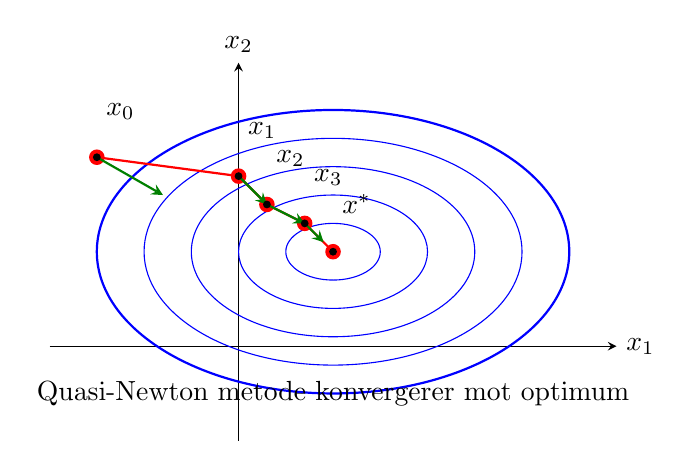
\begin{tikzpicture}[
      scale=1.2,
      >=stealth,
      point/.style={circle,fill=black,inner sep=1pt},
    ]

    % Koordinatsystem
    \draw[->] (-2,0) -- (4,0) node[right]{$x_1$};
    \draw[->] (0,-1) -- (0,3) node[above]{$x_2$};

    % Elliptiske nivålinjer for en kvadratisk funksjon
    \draw[blue, thick] (1,1) ellipse (2.5 and 1.5);
    \draw[blue] (1,1) ellipse (2 and 1.2);
    \draw[blue] (1,1) ellipse (1.5 and 0.9);
    \draw[blue] (1,1) ellipse (1 and 0.6);
    \draw[blue] (1,1) ellipse (0.5 and 0.3);

    % Optimeringsbane
    \draw[mark=*, red, thick, mark size=2pt] plot coordinates {
        (-1.5, 2)
        (0, 1.8)
        (0.3, 1.5)
        (0.7, 1.3)
        (1, 1)
      };

    % Gradient piler
    \draw[->, green!50!black, thick] (-1.5, 2) -- (-0.8, 1.6);
    \draw[->, green!50!black, thick] (0, 1.8) -- (0.3, 1.5);
    \draw[->, green!50!black, thick] (0.3, 1.5) -- (0.7, 1.3);
    \draw[->, green!50!black, thick] (0.7, 1.3) -- (0.9, 1.1);

    % Legg til punkter for tydelighet
    \node[point, label={[shift={(0.3,0.3)}]$\symbf{x}_0$}] at (-1.5, 2) {};
    \node[point, label={[shift={(0.3,0.3)}]$\symbf{x}_1$}] at (0, 1.8) {};
    \node[point, label={[shift={(0.3,0.3)}]$\symbf{x}_2$}] at (0.3, 1.5) {};
    \node[point, label={[shift={(0.3,0.3)}]$\symbf{x}_3$}] at (0.7, 1.3) {};
    \node[point, label={[shift={(0.3,0.3)}]$\symbf{x}^*$}] at (1, 1) {};

    % Figurtittel
    \node at (1, -0.5) {Quasi-Newton metode konvergerer mot optimum};

  \end{tikzpicture}
  \caption{Illustrasjon av Quasi-Newton-iterasjoner som konvergerer mot løsningen langs en ikke-lineær vei. De elliptiske konturene representerer nivålinjer for objektfunksjonen, og punktene viser iterasjonene fra \(\symbf{x}_0\) til den optimale løsningen \(\symbf{x}^*\).}
  \label{fig:quasi_newton_convergence}
\end{figure}

\subsection{Konvergens}
Under passende betingelser viser Quasi-Newton metoder superlineær konvergens:

\[
  \lim_{k \to \infty} \frac{\|\symbf{x}_{k+1} - \symbf{x}^*\|}{\|\symbf{x}_k - \symbf{x}^*\|} = 0
\]

Selv om denne konvergensraten er langsommere enn Newtons kvadratiske konvergens, er kostnaden per iterasjon betydelig lavere, noe som gir en mer effektiv algoritme totalt sett, spesielt for store problemer.

\subsection{Limited Memory BFGS (L-BFGS)}
For høydimensjonale problemer kan lagring av hele Hesse-approksimasjonen være uhåndterlig. Limited Memory BFGS (L-BFGS) lagrer kun de siste \(m\) parene \((\symbf{s}_k, \symbf{y}_k)\) og konstruerer approksimasjonen implisitt.

Dette gir en betydelig hukommelsesbesparelse samtidig som man beholder de gode konvergensegenskapene til BFGS-metoden.

\subsection{Fordeler og begrensninger}
\begin{itemize}
  \item \textbf{Fordeler}:
        \begin{itemize}
          \item Raskere enn gradientbaserte metoder
          \item Lavere kostnad per iterasjon enn Newtons metode
          \item Bygger opp kurvaturinformasjon iterativt
          \item Superlineær konvergens under passende betingelser
        \end{itemize}
  \item \textbf{Begrensninger}:
        \begin{itemize}
          \item Langsommere konvergens enn ren Newton-metode lokalt
          \item Kan kreve flere linjesøk
          \item Sensitiv til nøyaktigheten i linjesøket, spesielt for DFP
        \end{itemize}
\end{itemize}

For å sikre at Hesse-approksimasjonen forblir positiv definit, er det viktig at:

\begin{itemize}
  \item \(\symbf{y}_k^T\symbf{s}_k > 0\) (oppfylt under sterke Wolfe-betingelser)
  \item Initialmatrisen \(\symbf{B}_0\) eller \(\symbf{H}_0\) er positiv definit (ofte satt til \(\symbf{I}\))
\end{itemize}

En vanlig tilnærming for å forbedre ytelsen er å skalere den innledende approksimasjonen:

\[
  \symbf{H}_0 = \frac{\symbf{y}_k^T\symbf{s}_k}{\symbf{y}_k^T\symbf{y}_k}\symbf{I}
\]

Dette gir et bedre estimat for den faktiske skaleringen av den inverse Hesse-matrisen.

\chapter{Konveks optimering}

Hvis et optimeringsproblem er konvekst, kan vi være sikre på at vi finner en global optimal løsning.

\section*{Definisjoner}

\begin{definition}{Lineært optimeringsproblem}{linear_programming}
  Et lineært optimeringsproblem er et optimeringsproblem på formen
  \begin{align*}
    \text{minimer}     & \quad \min_{x \in \R^n} f(x)                \\
    \text{betinget av} & \quad h_i(x) \leq 0, \quad i = 1, \ldots, m \\
                       & \quad g_j(x) = 0, \quad j = 1, \ldots, p
  \end{align*}
  hvor \(f, h_i, g_j\) er lineære funksjoner.
\end{definition}

\begin{example}{Lineær funksjon}{linear_function}
  La \(f(\symbf{x}) = c^T\symbf{x} + d\) være en lineær funksjon, hvor \(c\) er en vektor normal til en hyperplan og \(d\) er en konstant.
  Da er \(f(\symbf{x}) = 0\) en lineær likning som definerer en hyperplan i \(\R^n\).
\end{example}

\begin{example}{Lineær regresjon}{linear_regression}
  La \(X \in \R^{n \times m}\) være en matrise med observasjoner og \(y \in \R^n\) være en vektor med målinger.
  Lineær regresjon er et eksempel på et lineært program hvor vi ønsker å finne en vektor \(w \in \R^m\) som minimerer kvadratfeilen
  \begin{equation*}
    \min_{w \in \R^m} \norm{Xw - y}_2^2.
  \end{equation*}
\end{example}

\section[Slaters betingelse]{\gls{slater-condition}}

\begin{definition}{Slater's Condition}{slater_condition}
  For a convex problem with inequality constraints
  \[
    c_i(x) \le 0,\quad i=1,2,\dots,m,
  \]
  Slater's condition holds if there exists an \(x\) such that
  \[
    c_i(x) < 0 \quad \text{for all } i.
  \]
\end{definition}

\begin{remark}{Intuition}{}
  This condition guarantees that the feasible region has a nonempty interior.

  In other words, the constraints are not all 'tight' at every point, which helps secure strong duality and the existence of Lagrange multipliers.
\end{remark}

\section[KKT-betingelser]{\gls{kkt-conditions}}

\begin{theorem}{KKT conditions}{kkt}
  \begin{align*}
    \mathcal{A}_1(x)            & := \{i \in \mathcal{I} \mid c_i(x) = 0\},                     \\
    \mathcal{A}_2(x)            & := \{1 \leq i \leq m \mid (Ax)_i = b_i\} \tag{Active indices} \\
    \text{Active indices at } x & \in \Omega                                                    \\
  \end{align*}

  \begin{itemize}
    \item \(A_i\) are the active constraints/indices at \(x\)
    \item \(C\) is the matrix of equality constraints.
    \item \(p\) is the direction of descent.
    \item \(x\) is the current point (feasible).
    \item \(T_{\Omega}(x)\) is the tangent cone at \(x\).
    \item \(c_i(x)\) is the value of the \(i\)-th constraint at \(x\).
    \item \(Ax\) is the value of the equality constraints at \(x\).
    \item \(b\) is the vector of equality constraints.
  \end{itemize}

  Assume that \emph{Slater's constraint} holds. Then, the following statements are equivalent:

  \begin{align*}
    p\in T_{\Omega}(x) & \Longleftrightarrow
    \begin{cases}
      \inner{\nabla c_i(x), p} \geq 0, & i \in \mathcal{A}_1(x) \\
      (Ax)_i \geq 0,                   & i \in \mathcal{A}_2(x) \\
      Cp = 0,                          &                        \\
    \end{cases}
  \end{align*}

\end{theorem}


\begin{lemma}{Farka's Lemma}{farkas_lemma}
  Let \(A \in \mathbb{R}^{m \times n}\) and \(c \in \mathbb{R}^n\). Then, exactly one of the following statements is true:
  \begin{enumerate}
    \item[] \((1)\) There exists an \(x \in \mathbb{R}^n\) such that \(Ax \preceq 0\) and \(c^T x < 0\).
    \item[] \((2)\) There exists a \(y \in \mathbb{R}^m\) such that \(A^T y + c = 0\) and \(y \succeq 0\).
  \end{enumerate}
\end{lemma}

\begin{proof}
  \begin{enumerate}
    \item[] Assume that \((1)\) holds. Then \(Ax = b\) and \(x \ge 0\). If there exists a \(y\) such that \(y^T A \ge 0\), then
          \[
            y^T b = y^T Ax = (y^T A)x \ge 0,
          \]
          which contradicts \(y^T b < 0\).
    \item[] Assume that \((1)\) does not hold. We want to show that \((2)\) holds.

          Let
          \[
            K = \{Ax \mid x \ge 0\}.
          \]
          Since \((1)\) does not hold, \(b \notin K\). Since \(K\) is a closed convex cone, by the separating hyperplane theorem, there exists a \(y \in \mathbb{R}^m\) such that
          \[
            y^T b < y^T z \quad \text{for all } z \in K.
          \]
          Since \(0 \in K\), we have \(y^T b < 0\).

          Now, for any \(x \ge 0\), we have \(Ax \in K\), so \(y^T b < y^T Ax\).

          Let \(x = e_i\), where \(e_i\) is the \(i\)-th standard basis vector. Then \(x \ge 0\), and
          \[
            y^T A e_i = (y^T A)_i > 0.
          \]
          Thus \(y^T A \ge 0\).
  \end{enumerate}

  \begin{center}
    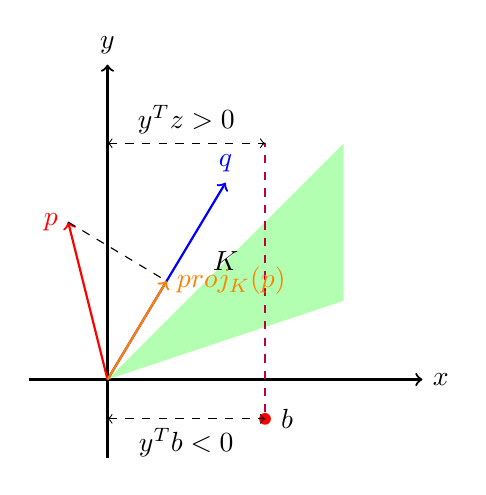
\begin{tikzpicture}
      \draw[->, thick] (-1, 0) -- (4, 0) node[right] {$x$};
      \draw[->, thick] (0, -1) -- (0, 4) node[above] {$y$};

      \fill[green!30] (0, 0) -- (3, 1) -- (3, 3) -- cycle;
      \node at (1.5, 1.5) {$K$};

      \node[circle, fill=red, inner sep=1.5pt, label=right:$b$] (b) at (2, -0.5) {};

      \draw[dashed, purple] (b) -- (2, 3);
      \draw[<->, dashed, black] (0, -0.5) -- (2, -0.5) node[midway, below, black] {$y^Tb < 0$};
      \draw[<->, dashed, black] (0, 3) -- (2, 3) node[midway, above, black] {$y^Tz > 0$};

      % Adding new vectors
      \draw[->, thick, blue] (0, 0) -- (1.5, 2.5) node[above] {$q$};
      \draw[->, thick, red] (0, 0) -- (-0.5, 2) node[left] {$p$};
      \draw[->, thick, orange] (0, 0) -- (0.75, 1.25) node[right] {$proj_K(p)$};
      \draw[dashed] (-0.5, 2) -- (0.75, 1.25);
    \end{tikzpicture}
  \end{center}

  The figure illustrates the geometric interpretation of Farkas' Lemma. The green region $K$ represents the cone of feasible points $\{Ax \mid x \ge 0\}$. The point $b$ (in red) lies outside this cone. The purple dashed line represents the separating hyperplane, which separates $b$ from $K$. Vector $p$ (in red) is projected onto the cone $K$, resulting in $proj_K(p)$ (in orange). Vector $q$ (in blue) lies inside the cone $K$. The black dashed lines show that the inner product $y^Tb$ is negative, while the inner product $y^Tz$ is positive for points $z$ in the cone $K$.

\end{proof}


\begin{theorem}{KKT conditions}{kkt_conditions}
  Assume \(c_i, i \in \mathcal{I}\) are concave in \(\mathcal{C}^1\),
  \(A\in \mathbb{R}^{m \times d}, b \in \mathbb{R}^m\) and \(C\in \mathbb{R}^{l \times d}\) and that \(f:\mathbb{R}^d \to \mathbb{R}\) is \(\mathcal{C}^1\). Assume that \emph{Slater's condition} holds.

  If \(x^\star\) is a local minimum of \(\min_x f(x)\) s.t.
  \[
    \begin{cases}
      c_i(x) \geq 0, & \forall i \in \mathcal{I} \\
      Ax \geq b,     &                           \\
      Cx = b,        &
    \end{cases}
  \]
  then there exists a \emph{Lagrange multipliers} \(\lambda^\star, \mu^\star\) with \(v \in \R^e\) s.t. the \emph{KKT conditions} hold:

  Then, the following statements are equivalent:
  \begin{align}
    \nabla f(x^\star) = \sum_{i\in \mathcal{I}} \lambda_i^\star \nabla c_i(x^\star) + A^T \mu^\star + C^T v^\star \\
    \begin{cases}
      c_i(x^\star) \geq 0, & \forall i \in \mathcal{I} \\
      Ax^\star \geq b,     &                           \\
      Cx^\star = e,        &                           \\
    \end{cases} \tag{Feasibility}                                                              \\
    \begin{cases}
      \lambda_i^\star \geq 0, & \forall i \in \mathcal{I} \\
      \mu_j^\star \in \geq 0, & \forall j \in \mathcal{J} \\
    \end{cases} \tag{Dual feasibility}                                                           \\
    \begin{cases}
      \lambda_i^\star c_i(x^\star) = 0, & \forall i \in \mathcal{I} \\
      \mu_j^\star C_j^T = 0,            & \forall j \in \mathcal{J} \\
    \end{cases} \tag{Complementary slackness}                                                 \\
    \begin{cases}
      \lambda_i^\star c_i(x^\star) = 0,      & \forall i \in \mathcal{I} \\
      \inner{\mu_j^\star, Ax^\star - b} = 0, & \forall j \in \mathcal{J} \\
    \end{cases} \tag{Complementary slackness}
  \end{align}
\end{theorem}

\begin{proof}{}{}
  We have the optimality condition:
  \[
    \inner{\nabla f(x^\star), p} \geq 0 \, \forall p \in T_{\Omega}(x^\star)
  \]
  \medskip
  \begin{align*}
    p \in T_{\Omega}(x^\star) \iff
    \begin{cases}
      \inner{\nabla c_i (x^\star), p }\geq 0 & \forall i \in \mathcal{A}_1(x^\star)                         \\
      \text{or: there does not exist any } p \in \R^d \text{ such that:} & \\
      \begin{cases}
        \inner{\nabla c_i (x^\star), p }\geq 0 & \forall i \in \mathcal{A}_1(x^\star) \\
        \inner{A_i^T , p }\geq 0               & \forall i \in \mathcal{A}_2(x^\star) \\
        \inner{ (C_i )^T, p } = 0              & \forall 1 \leq i \leq l              \\
        \inner{\nabla f (x^\star), p } < 0     & 
      \end{cases}                             \\
      (Ap)_i \geq 0 & \forall i \in \mathcal{A}_2(x^\star)                                                      \\
      Cp = 0        &
    \end{cases}
  \end{align*}

  The second alternative is Farka's Lemma does not hold \(\implies\) The first holds.

  \begin{align*}
    \nabla f(x^\star) & = \sum_{i\in \mathcal{A}_1(x^\star)} \lambda_i^\star \nabla c_i(x^\star) + \sum_{i \in \mathcal{A}_2(x^\star)} \mu_i^\star A_i^T + \sum_{i=1}^l v_i^\star C_i^T \\
  \end{align*}

  For some  \(\lambda_i^\star \geq 0, \mu_i^\star \geq 0, v_i^\star \in \R\).

  Now define: \(\lambda_i^\star = 0 \) for \(i \notin \mathcal{A}_1(x^\star)\) and \(\mu_i^\star = 0\) for \(i \notin \mathcal{A}_2(x^\star)\).

  Then we have:
  \begin{align*}
    \nabla f(x^\star) & = \sum_{i\in \mathcal{I}} \lambda_i^\star \nabla c_i(x^\star) + \sum_{1 \leq i \leq m} \mu_i^\star A_i^T + \sum_{1 \leq i \leq l} v_i^\star C_i^T = \text{(1)} \\
  \end{align*}
  \qed
\end{proof}

\begin{definition}{The Lagrangian of a problem}{lagrangian}
  The Lagrangian of a problem is the function \(\mathcal{L}: \mathbb{R}^d \times \mathbb{R}^m \times \mathbb{R}^l \times \mathbb{R}^e \to \mathbb{R}\) defined as:
  \begin{align*}
    \mathcal{L}(x, \lambda, \mu, v) &= f(x) + \sum_{i\in \mathcal{I}} \lambda_i c_i(x) + \sum_{1 \leq i \leq m} \mu_i (Ax - b)_i + \sum_{1 \leq i \leq l} v_i (Cx - b)_i \\
    &= f(x) - \sum_{i \in \mathcal{I}} \lambda_i c_i(x) - \inner{\mu, Ax - b} - \inner{v, Cx - e}\footnote{\( (1) \iff \nabla_x \mathcal{L}(x, \lambda, \mu, v) = 0\)}
  \end{align*}

\end{definition}

\clearpage

\appendix
\include{preamble/appendix/AlgorithmMap}
\chapter{Formeltabell}

\begin{table}[ht]
  \centering
  \footnotesize
  \begin{tabularx}{\textwidth}{@{}>{\color{black!70}}l>{\raggedright\arraybackslash}X@{}}
    \toprule
    \rowcolor{headerblue}
    \textbf{Term}     & \textbf{Definition/Formula}                                                                                                                               \\
    \midrule

    Convex            & \( f(\lambda x + (1-\lambda)y) \leq \lambda f(x) + (1-\lambda)f(y), \ \forall x,y \in \R^d, \lambda \in [0,1] \)                                          \\

    Coercive          & \( \lim_{\|x\| \to \infty} f(x) = \infty \) (ensures existence of minima)                                                                                 \\

    lsc               & \( \liminf_{x \to x_0} f(x) \geq f(x_0) \) (sublevel sets closed)                                                                                         \\

    Quasi-Convex      & \( \mathcal{L}_{f}(\alpha) = \{x \mid f(x) \leq \alpha\} \text{ convex } \forall \alpha \in \R \iff f(\lambda x + (1-\lambda)y) \leq \max\{f(x),f(y)\} \) \\

    Local Minimum     & \( \exists \epsilon > 0: f(x^*) \leq f(x), \, \forall x \in B_\epsilon(x^*) \)                                                                            \\

    Global Minimum    & \( f(x^*) \leq f(x), \, \forall x \in \R^d \)                                                                                                             \\

    Proximal Operator & \( \text{prox}_{\gamma f}(v) = \arg\min_x \left( f(x) + \frac{1}{2\gamma}\|x - v\|^2 \right) \)                                                           \\

    Subgradient       & \( g \in \partial f(x) \text{ if } f(y) \geq f(x) + g^\top(y-x), \, \forall y \in \R^d \)                                                                 \\

    Stochastic GD     & \( x_{k+1} = x_k - \eta_k \nabla f_{i_k}(x_k) \) (randomized gradients)                                                                                   \\

    Newton's Method   & \( x_{k+1} = x_k - [\nabla^2 f(x_k)]^{-1} \nabla f(x_k) \)                                                                                                \\
    \bottomrule
  \end{tabularx}
  \caption{Quick Reference: Key Definitions and Formulas}
\end{table}

\include{preamble/appendix/Functions}
\include{preamble/appendix/LectureNotes}

\printbibliography
\printglossary
\printglossary[type=\acronymtype]

\end{document}
